\documentclass[UKenglish]{beamer}

\usepackage[T1]{fontenc}

\usepackage{graphicx}

\usepackage[normalem]{ulem}

\usepackage{newclude}

% Haskell
\usepackage[cache=false]{minted}

\usepackage{tikz}
% Overlay effec
\usetikzlibrary{shapes.geometric,positioning,shapes.symbols,overlay-beamer-styles}

%% UIB
\usepackage[utf8]{inputenx} % For æ, ø, å
\usepackage{csquotes}       % Quotation marks
\usepackage{microtype}      % Improved typography
\usepackage{amssymb}        % Mathematical symbols
\usepackage{mathtools}      % Mathematical symbols
\usepackage[absolute, overlay]{textpos} % Arbitrary placement
\setlength{\TPHorizModule}{\paperwidth} % Textpos units
\setlength{\TPVertModule}{\paperheight} % Textpos units
%%

\title{What is an IDE?}
\author{Nils Michael Fitjar}
\date{\today}

\begin{document}

\frame{\titlepage}

\section{Project}
\begin{frame}{Project}
  Create a modular IDE.
  (modular in this context, meaning it can be extended with plugins)
\end{frame}

\section{Showcase}
\begin{frame}{IDE}
  So, here is my IDE:
\end{frame}

\begin{frame}{IDE Features}
  \begin{itemize}
    \item Dynamically loading of Plugins
  \end{itemize}
\end{frame}

\section{Plugins}
\begin{frame}{Loading of Plugins}
  A Plugin, is a shared-object-file, that is dynamically loaded
  during startup.
  It needs to expose, an init, view and update function.
\end{frame}

\begin{frame}{Plugin Example}
  \begin{minted}{haskell}
-- Manifest :: Map
init :: Map
init :: [("counter", ValInt 0)]

update :: Msg -> Map -> Map
update (PluginMsg "counter") model =
  case lookup "counter" model of
    Just (ValInt i) -> insert "counter" (ValInt (i + 1)) model
    Nothing -> insert "counter" (ValInt 0) model

view :: Map -> Html
view model = Div [] [Text "Hello, World!"
  , Btn [OnClick (PluginMsg "counter")] []
  , Text (putStrLn (lookupOrDefault "counter" model))
\end{minted}



\end{frame}

\begin{frame}{What is an IDE?}
  \begin{enumerate}
    \item Before Woke: Text editor and a compiler.
    \item After Woke: Text editor, Debugger, File Explorer,
    Syntax Highlighting, LSP, Compiler/Interpreter, Linter, Integrated-VCS,
    Themes, Integrated-Terminal, Workspace, Language Agnostic, Easy Setup, AI
    and more
  \end{enumerate}
\end{frame}

\begin{frame}{What is a Text Editor?}
  \begin{itemize}
    \item A file is just a string of bytes
    \item Need some form of abstraction on this to achieve a standard text
    editor movement
    \item You can group them by newlines
    \item But your syntax highlighter might want a different representation of the text
    \begin{itemize}
      \item Like grouping multi-line-comments
      \item \begin{minted}{haskell}
-- Single line comment

{-
Multi-line-comment
-}
\end{minted}


    \end{itemize}
  \end{itemize}
\end{frame}

\begin{frame}{Example Text Editor Parts*}
  \center
  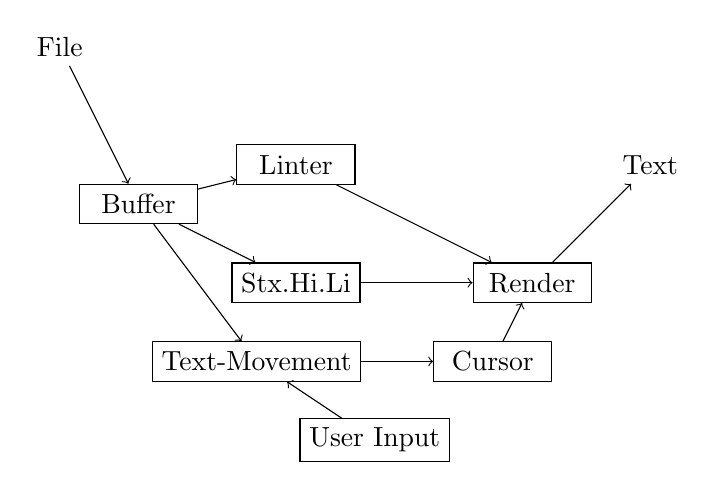
\begin{tikzpicture}
  % Nodes
  \node (file) [] at (-6, 3) {File};
  \node (parser) [rectangle, draw, minimum height=0.5cm, minimum width=1.5cm] at (-5, 1) {Buffer};
  \node (stxhili) [rectangle, draw, minimum height=0.5cm, minimum width=1.5cm] at (-3, 0) {Stx.Hi.Li};
  \node (text-movement) [rectangle, draw, minimum height=0.5cm, minimum width=1.5cm] at (-3.5, -1) {Text-Movement};
  \node (linter) [rectangle, draw, minimum height=0.5cm, minimum width=1.5cm] at (-3, 1.5) {Linter};
  \node (cursor) [rectangle, draw, minimum height=0.5cm, minimum width=1.5cm] at (-0.5, -1) {Cursor};
  \node (user-input) [rectangle, draw, minimum height=0.5cm, minimum width=1.5cm] at (-2, -2) {User Input};
  \node (render) [rectangle, draw, minimum height=0.5cm, minimum width=1.5cm] at (0, 0) {Render};
  \node (text) at (1.5, 1.5) {Text};
  % Arrow
  \draw[->] (file) -- (parser) node[midway, above] {};
  \draw[->] (parser) -- (stxhili) node[midway, above] {};
  \draw[->] (parser) -- (linter) node[midway, above] {};
  \draw[->] (parser) -- (text-movement) node[midway, above] {};
  \draw[<-] (render) -- (stxhili) node[midway, above] {};
  \draw[<-] (render) -- (linter) node[midway, above] {};
  \draw[<-] (cursor) -- (text-movement) node[midway, above] {};
  \draw[<-] (text-movement) -- (user-input) node[midway, above] {};
  \draw[->] (cursor) -- (render) node[midway, above] {};
  \draw[->] (render) -- (text) node[midway, above] {};
\end{tikzpicture}


\end{frame}

\begin{frame}{Example Text Movement}
  \begin{itemize}
    \item Can move by individual symbols, words, lines, pages
    \begin{enumerate}
      \item Group by individual symbols
      \item Group symbols by word
      \item Group words by line
      \item Group line by page
    \end{enumerate}
    \item Can jump to symbol at start/end of word, line, page
  \end{itemize}
\end{frame}

\begin{frame}{What's missing?}
  \begin{itemize}
    \item For the text editor: editing of text
    \begin{itemize}
      \item Saving
      \item Opening
      \item Closing
      \item Deleting
    \end{itemize}
  \end{itemize}
\end{frame}

\end{document}
